\documentclass[11pt,a4paper]{article}
\usepackage[spanish,es-nodecimaldot]{babel}	% Utilizar español
\usepackage[utf8]{inputenc}					% Caracteres UTF-8
\usepackage{graphicx}						% Imagenes
\usepackage[hidelinks]{hyperref}			% Poner enlaces sin marcarlos en rojo
\usepackage{fancyhdr}						% Modificar encabezados y pies de pagina
\usepackage{float}							% Insertar figuras
\usepackage[textwidth=390pt]{geometry}		% Anchura de la pagina
\usepackage[nottoc]{tocbibind}				% Referencias (no incluir num pagina indice en Indice)
\usepackage{enumitem}						% Permitir enumerate con distintos simbolos
\usepackage[T1]{fontenc}					% Usar textsc en sections
\usepackage{amsmath}						% Símbolos matemáticos

% Comando para poner el nombre de la asignatura
\newcommand{\asignatura}{Visión por Computador}
\newcommand{\autor}{Vladislav Nikolov Vasilev}
\newcommand{\titulo}{Trabajo 3}
\newcommand{\subtitulo}{Cuestiones de teoría}

\newcommand{\answer}{\noindent\textbf{Solución}}
\newcommand{\question}[1]{\noindent\textbf{#1}}
\newcommand{\nonumsection}[1]{\section*{#1}\addcontentsline{toc}{section}{#1}}

% Configuracion de encabezados y pies de pagina
\pagestyle{fancy}
\lhead{\autor{}}
\rhead{\asignatura{}}
\lfoot{Grado en Ingeniería Informática}
\cfoot{}
\rfoot{\thepage}
\renewcommand{\headrulewidth}{0.4pt}		% Linea cabeza de pagina
\renewcommand{\footrulewidth}{0.4pt}		% Linea pie de pagina

\begin{document}
\pagenumbering{gobble}

% Pagina de titulo
\begin{titlepage}

\begin{minipage}{\textwidth}

\centering

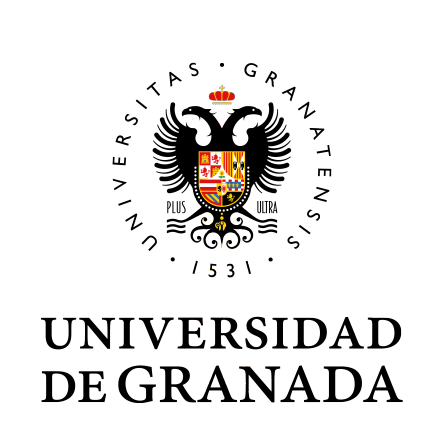
\includegraphics[scale=0.5]{img/ugr.png}\\

\textsc{\Large \asignatura{}\\[0.2cm]}
\textsc{GRADO EN INGENIERÍA INFORMÁTICA}\\[1cm]

\noindent\rule[-1ex]{\textwidth}{1pt}\\[1.5ex]
\textsc{{\Huge \titulo\\[0.5ex]}}
\textsc{{\Large \subtitulo\\}}
\noindent\rule[-1ex]{\textwidth}{2pt}\\[3.5ex]

\end{minipage}

\vspace{0.5cm}

\begin{minipage}{\textwidth}

\centering

\textbf{Autor}\\ {\autor{}}\\[2.5ex]
\textbf{Rama}\\ {Computación y Sistemas Inteligentes}\\[2.5ex]
\vspace{0.3cm}


\includegraphics[scale=0.3]{img/etsiit.jpeg}

\vspace{0.7cm}
\textsc{Escuela Técnica Superior de Ingenierías Informática y de Telecomunicación}\\
\vspace{1cm}
\textsc{Curso 2019-2020}
\end{minipage}
\end{titlepage}

\pagenumbering{arabic}
\tableofcontents
\thispagestyle{empty}				% No usar estilo en la pagina de indice

\newpage

\setlength{\parskip}{1em}

\nonumsection{Ejercicio 1}

\question{¿Cuál es la transformación más fuerte de la geometría de una
escena que puede introducirse al tomar una foto de ella? Dar algún
ejemplo.}

\answer

\nonumsection{Ejercicio 2}

\question{¿Por qué es necesario usar el plano proyectivo para estudiar las
transformaciones en las imágenes de fotos de escenas? Dar algún
ejemplo.}

\answer

\nonumsection{Ejercicio 3}

\question{Sabemos que en el plano proyectivo un punto no existe en el
sentido del plano afín, sino que se define por una clase de
equivalencia de vectores definida por $\lbrace k(x,y,1),k \neq 0 \rbrace$. Razone usando
las coordenadas proyectivas de los puntos afines de una recta que
pase por el $(0,0)$ del plano afín y verifique que los punto de la
recta del infinito del plano proyectivo son necsariamente vectores
del tipo $(*,*,0)$ con $*=$cualquier número.}

\answer

\nonumsection{Ejercicio 4}

\question{¿Qué propiedades de la geometría de un plano quedan invariantes
cuando se toma una foto de él? Justificar la respuesta.}

\answer

\nonumsection{Ejercicio 5}



\nonumsection{Ejercicio 6}

\question{¿Cuál es el mínimo número de escalares necesarios para fijar
una homografía general? ¿Y si la homografía es afín? Justificar la
respuesta.}

\answer

\nonumsection{Ejercicio 7}

\question{Defina una homografía entre planos proyectivos que haga que el
punto $(3,0,2)$ del plano proyectivo-1 se transforme en un punto de
la recta del infinito del plano proyectivo-2? Justificar la
respuesta.}

\answer

\nonumsection{Ejercicio 8}



\nonumsection{Ejercicio 9}

\question{¿Cuáles son las propiedades necesarias y suficientes para que
una matriz defina un movimiento geométrico no degenerado entre
planos? Justificar la respuesta.}

\answer

\nonumsection{Ejercicio 10}

\question{¿Qué información de la imagen usa el detector de Harris para
seleccionar puntos? ¿El detector de Harris detecta patrones
geométricos o fotométricos? Justificar la contestación.}

\answer

\nonumsection{Ejercicio 11}

\question{¿Sería adecuado usar como descriptor de un punto Harris los
valores de los píxeles de su región de soporte? Identifique
ventajas, inconvenientes y mecanismos de superación de estos
últimos.}

\answer

\nonumsection{Ejercicio 12}

\question{Describa un par de criterios que sirvan para seleccionar
parejas de puntos en correspondencias (``matching'') a partir de
descriptores de regiones extraídos de dos imágenes. ¿Por qué no es
posible garantizar que todas las parejas son correctas?}

\answer

\nonumsection{Ejercicio 13}

\question{¿Cuál es el objetivo principal del uso de la técnica RANSAC en
el cálculo de una homografía? Justificar la respuesta.}

\answer

\nonumsection{Ejercicio 14}

\question{Si tengo 4 imágenes de una escena de manera que se solapan la
1-2, 2-3 y 3-4. ¿Cuál es el número mínimo de parejas de puntos en
correspondencias necesarios para montar un mosaico? Justificar la
respuesta.}

\answer

\nonumsection{Ejercicio 15}

\question{¿En la confección de un mosaico con proyección rectangular es
esperable que aparezcan deformaciones geométricas de la escena
real? ¿Cuáles y por qué? ¿Bajo qué condiciones esas deformaciones
podrían no estar presentes? Justificar la respuesta.}

\answer

\newpage

\begin{thebibliography}{5}

\end{thebibliography}

\end{document}

